\newpage
\changeindent{0cm}
\section{要素技術}
\changeindent{2cm}

本章では, 本研究に関連する要素技術についての説明をする.

\subsection{Knowledge Graph}

本節では, Knowledge Graph というデータ構造について説明する. なお, Knowledge Graph に一意の定義は存在しないため, 本研究に用いた Knowledge Graph の定義についてのみ詳説する. \par

\subsubsection{概要}

本研究で扱う Knowledge Graph は, さまざまな情報やデータから抽出した知識をグラフ構造上に整理した知識ベースの一種である. Google により実世界のオブジェクトの検索を可能にするものとして紹介され, さまざまな研究や産業分野に急速に普及された \cite{google_knowledge_graph}. \par
図 \ref{kg} に Knowledge Graph の例を示す. Knowledge Graph は, それぞれ意味をもつ Entity (実体) 集合と, その Entity 同士の関係性を表現する Relation (関係) 集合によって構成され, それぞれが図 \ref{kg} のグラフにおけるノードとエッジの役目を担っている. \par

\begin{figure}[h]
    \centering
    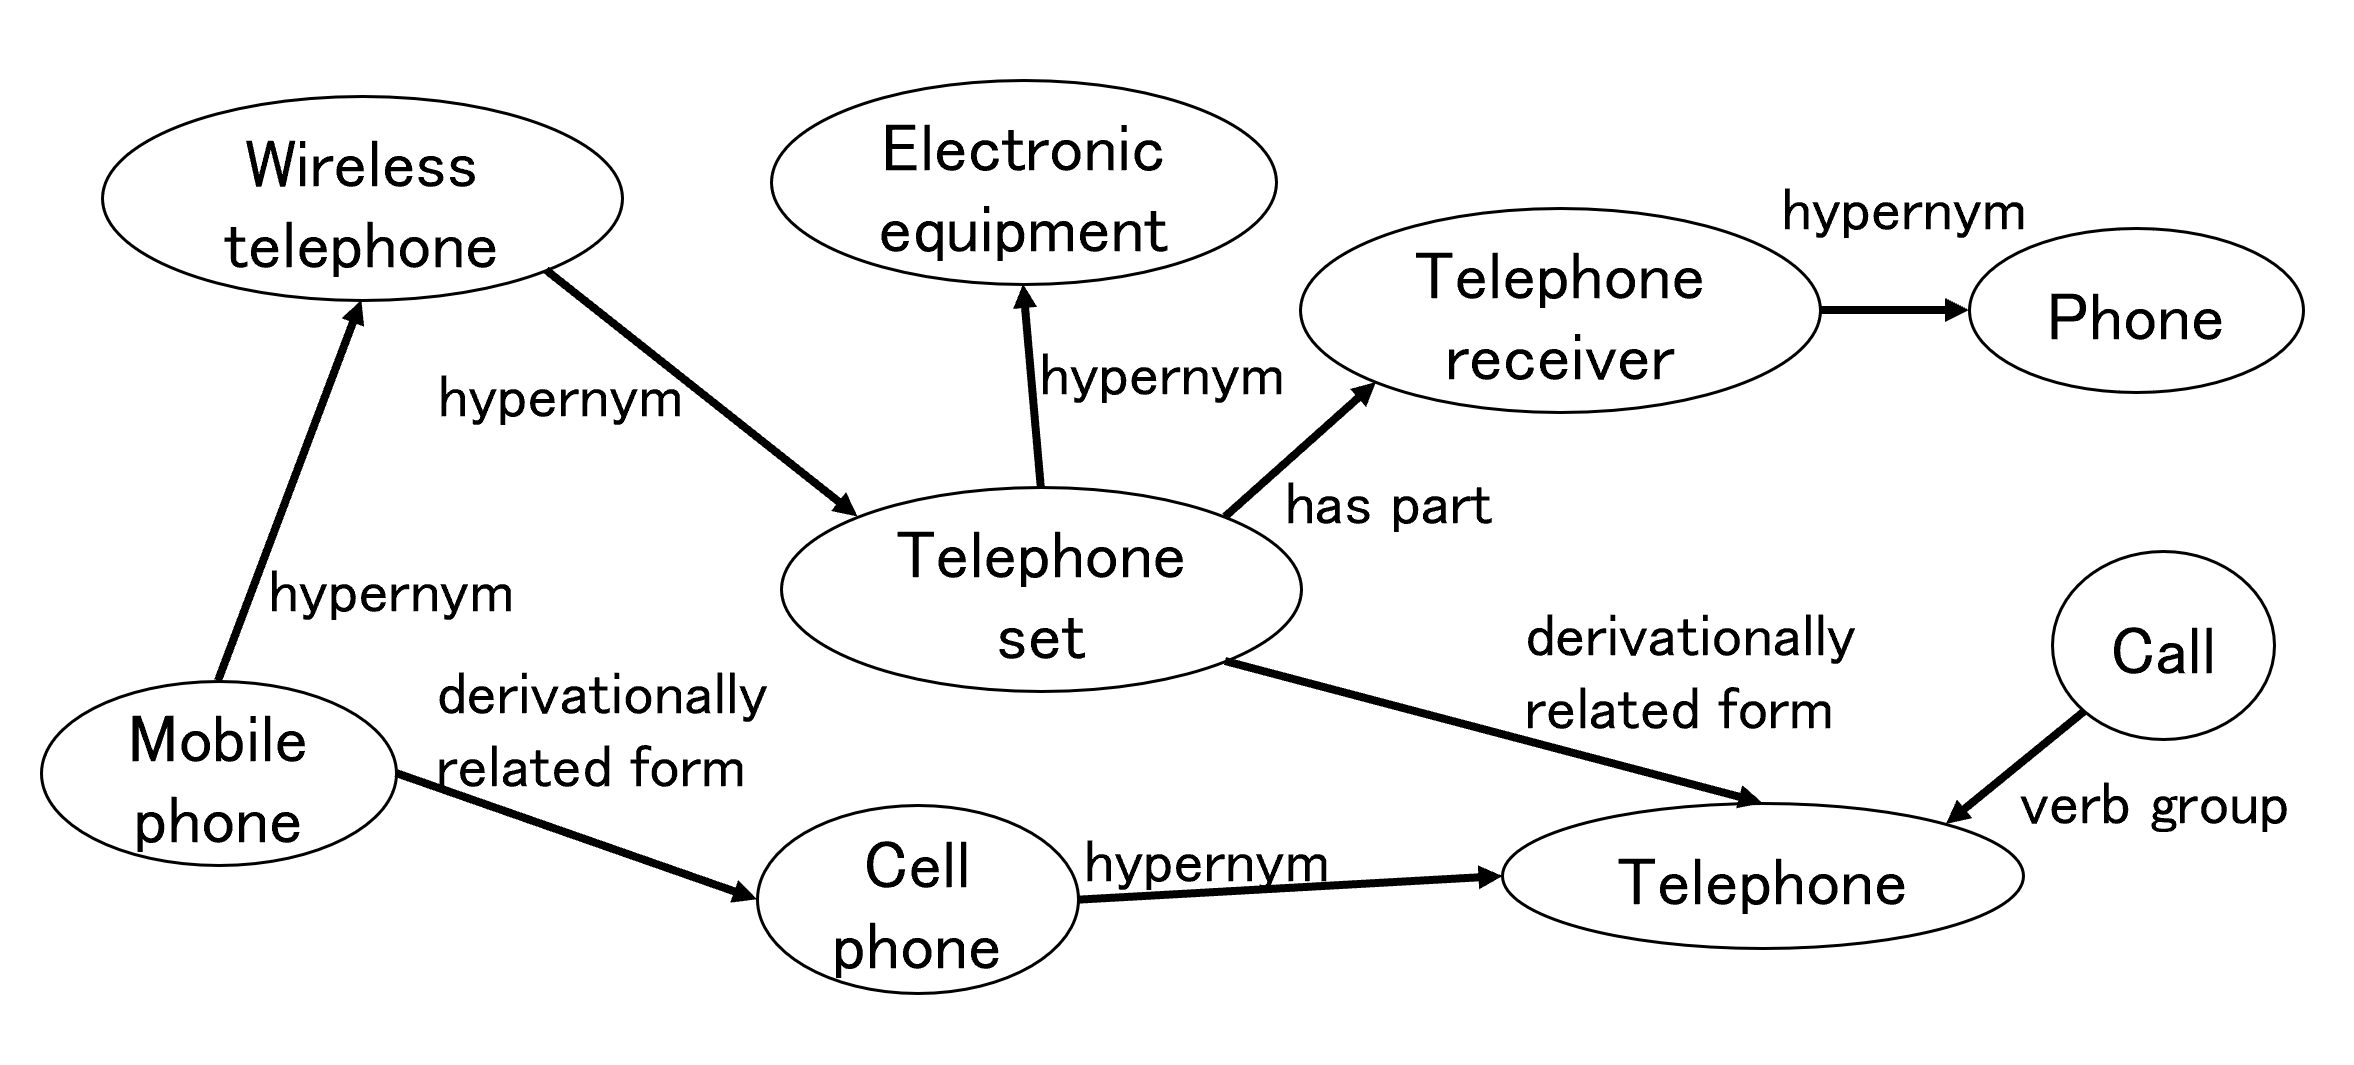
\includegraphics[width=16cm]{assets/Ex_KG.png}
    \caption{Knowledge Graph の例}
    \label{kg}
\end{figure}

\subsubsection{データ構造}

Knowledge Graph はその要素として Entity 集合と Relation 集合をもつ. Entity 集合は, 人物, 場所, 単語, 文といった, 何らかの属性をもつ ``Entity" の集合である. 各 Entity がもつ属性の種類は, 有限の属性だけでなく, 実数値や自然言語文などの非有限のものもある. なお, 全く同じ属性をもつ異なる Entity は存在しない. \par
続いて, Relation 集合は 2 つの Entity に対して, 一方の Entity から見た Entity との関係性を規定する ``Relation" の集合である. Relation によって個々の Entity に繋がりを与えて, それにより全体として有用な意味をもつネットワークができる. 各 Relation は Entity と同様に属性をもち, それにより Entity 同士の関係を細かく規定する. なお, Relation のもつ属性は有限の属性に限定される. \par

\subsubsection{グラフ表現}

Knowledge Graph はグラフとして表現できる. 図 \ref{kg} の Knowledge Graph のグラフを例として説明する. 図 \ref{kg} の Knowledge Graph は, WordNet の一部を Knowledge Graph として表現した一例である. Knowledge Graph をグラフとして表現する際には一般的に, Entity をグラフにおけるノード, Relation をグラフにおけるエッジとする. このようにして構成されるため, このグラフはノードおよびエッジの属性をもつ. また, 2 つの Entity の間に複数の関係がある場合は, 2 つの Entity の間に複数の Relation が与えられる. そのため, Knowledge Graph をグラフとして表現したものは重み付き多重グラフであるといえる. \par
図 \ref{kg} に示すグラフにおけるノードが Entity であり, エッジが Relation となる. すなわち, この Knowledge Graph は ``Wireless telephone", ``Telephone set", ``Telephone", ``Call" などの Entity をもち, ``hypernym", ``has part", ``verb group", ``derivationally related form" の 4 種類の Relation をもつ. この Knowledge Graph は WordNet \cite{Wordnet} を Knowledge Graph として表現した一例であるため, 各 Entity は属性として WordNet の各見出し語の単語をもつ. そして, Relation によってそれらの単語の関係が規定されている. 例として, ``hypernym" という Relation は単語間の上位下位の関係を規定するものである. そして, 図 \ref{kg} では, この属性をもつ Relation によって ``Wireless telephone" から ``Telephone set" へと繋がれている. この 2 つの Entity と 1 つの Relation によって,「``Wireless telephone" の上位語は ``Telephone set"」という関係が定まる. \par

\subsubsection{Triple}

グラフとは異なる表現として, Relation で繋がれた 2 つの Entity に着目し, 2 つの Entity とそれを結ぶ Relation をひとまとめにした Triple の集合として表現する事もできる. 表 \ref{Triple} に Knowledge Graph を Triple として表現した例を示す. 表 \ref{Triple} は, 図 \ref{kg} の一部の情報を Triple で表現している. \par
それぞれの Triple は, Relation の出発元の Entity, Relation, 向かう先の Entity をもつ. それぞれを Head, Relation, Tail と呼ぶ. 本研究では, 主に Triple 表現を利用する. \par

\begin{table}[h]
    \centering
    \caption{Knowledge Graph の Triple 表現}
    \label{Triple}
    \begin{tabular}{|c|c|c|} \hline
      Head & Relation & Tail \\ \hline \hline
      Wireless telephone & hypernym & Telephone set \\ \hline
      Telephone set & derivationally related form & Telephone \\ \hline
      Telephone set& has part & Telephone receiver \\ \hline
      Call & verb group & Telephone \\ \hline
      Mobile phone & hypernym & Wireless telephone \\ \hline
      \vdots & \vdots & \vdots \\ \hline
    \end{tabular}
\end{table}

\subsubsection{埋め込み手法}

Knowledge Graph はその要素として Entity 集合, Relation 集合をもち, それらは実数値や自然言語文などの属性をもつ. しかし Knowledge Graph を計算機で扱う上で, さまざまな種類のデータによって構成されたそれらをそのまま用いることは容易ではない. そこで, 自然言語処理と同様に, Knowledge Graph の各要素を埋め込み表現にするさまざまな手法が考案されてきた. それらのうち代表的なものをいくつか紹介する. Knowledge Graph 埋め込みの手法を大きく分類すると, 以下の 3 つの種類がある \cite{Embedding}. \par

\begin{description}
   \item[行列変換に基づく手法]\mbox{}\\
     \quad 行列変換に基づく手法は, Triple の隣接行列を分解することで, Entity や Relation を表す埋め込み表現を得る. すなわち, $n = |{\rm Entity}|$ 個の Entity と $m = |{\rm Relation}|$ 個の Relation によって構成される Knowledge Graph の隣接行列 $V \in \mathbb{R}^{n \times n}, v_{x,y} \in \{0, 1, \ldots, m-1 \}$ を分解して, 各 Entity, Relation を埋め込み表現にする手法である. \par
    \quad これに分類される埋め込み表現獲得手法としては, RESCAL \cite{RESCAL}, DistMult \cite{DistMult}, HolE \cite{HolE}, 複素数空間を用いる ComplEx \cite{ComplEx} などがある. \par
   \item[ベクトルの移動に基づく手法]\mbox{}\\
	\quad ベクトルの移動に基づく手法は, Entity や Relation の埋め込み表現を, 各 Triple, あるいは存在しない偽物の Triple に含まれる Head, Relation, Tail の埋め込み表現のベクトル演算によって score を算出して, その score が条件を満たすように最適化することでもっともらしい埋め込み表現を得る. \par
    \quad これに分類される埋め込み表現獲得手法の 1 つとして, TransE \cite{TransE_WN18} があり, これを例に説明する. TransE は, 各 Entity および各 Relation をそれぞれ $d$ 次元の埋め込み表現にする. TransE は Triple を構成する Head, Relation, Tail のそれぞれの埋め込み表現 $\bm{v}_{\rm Head}, \bm{v}_{\rm Relation}, \bm{v}_{\rm Tail}$ に対して, 各 Triple が $\bm{v}_{\rm Head} + \bm{v}_{\rm Relation} = \bm{v}_{\rm Tail}$ を満たすように埋め込み表現を学習する手法である. このとき, score は $\bm{v}_{\rm Head} + \bm{v}_{\rm Relation}$ と $\bm{v}_{\rm Tail}$ の乖離であり, 式で表すと
    \begin{equation}
        {\rm score} = −||\bm{v}_{\rm Head} + \bm{v}_{\rm Relation} − \bm{v}_{\rm Tail}||
    \end{equation}
    と定義される. この score の値が正例の Triple に対して最大化して負例の Triple に対して最小化するように, 誤差逆伝播法を用いて埋め込み表現を学習する. \par
    \quad このように, 埋め込み表現に対する演算によって score を算出して, より良い score が得られるように埋め込み表現を学習していく. TransE 以外の手法としては, TransE を改良した ITransE \cite{ITransE}, TransH \cite{TransH}, TransR \cite{TransR}, PTransE \cite{PTransE}, 複素数ベクトルを用いてその回転を利用する手法である RotatE \cite{RotatE} がある. さらに, 階層構造や木構造をうまく扱うことを期待してユークリッド空間ではなくポアンカレ空間 \cite{Poincare} に埋め込む Poincare Embedding \cite{Poincar_Embedding} を用いる手法の RotH \cite{AttH_etc}, AttH \cite{AttH_etc} がある. \par
   \item[ニューラルネットワークに基づく手法]\mbox{}\\
	\quad ニューラルネットワークに基づく手法は, Entity や Relation の埋め込み表現をニューラルネットワークによって最適化することで埋め込み表現を得る. \par
    \quad これに分類される埋め込み表現獲得手法としては, 畳み込み器 \cite{Convolutional} を用いて Head と Relation から Tail の埋め込み表現を推定し, 訓練データにより埋め込み表現を最適化する ConvE \cite{WN18RR_ConvE}, 階層型 Transformer によって Triple の関係と各 Entity のもつすべての Triple の情報をモデルに入力とすることで, 複雑な関係が含まれた Knowledge Graph に対応する HittER \cite{HittER} などがある. \par
    \quad また, Knowledge Graph に限定せず人間関係, Web ページのリンク, 道路交通網, 化学結合といったさまざまなグラフを埋め込むグラフニューラルネットワーク (Graph Neural Networks, GNN) \cite{GNN} についてもさまざまなものが提案されている. 代表的なものとしては, グラフ構造を畳み込む Relational Graph Convolutional Networks (R-GCN) \cite{R-GCN}, GNN に Attention 機構を導入した Graph Attention Networks (GAN) \cite{GAN} などがある. また, R-GCN を Knowledge Graph に応用し, 購買推薦システムに用いる KGCN \cite{KGCN} も提案されている. \par
\end{description}

\subsubsection{活用例}

Knowledge Graph はさまざまな種類のデータを統合的にグラフとして扱う. これにより, 一度に多元的な情報を得ることができる. Knowledge Graph が利用されているものとして最も有名なものが Google Knowledge Graph である. これは Google が保有する各情報を Entity として, それぞれが Relation によって紐付けられた Knowledge Graph である. これを用いることでユーザーはある情報について検索した際にそれに付随する人や場所や物事等に関する多角的な情報を得ることができる. \par
また近年, Knowledge Graph を機械学習に用いることによってさまざまなデータ間の複雑なつながりを学習する事への期待が高まっている \cite{recommend_system}. 例えば過去の売買履歴や商品データによる購買推薦システムを作る際に Knowledge Graph を用いることで, 顧客の購入履歴や品物の種類といったデータを総合的に扱い, 商品と顧客のつながりを学習することができる. この際に, 推論の根拠となる Entity や Relation の明確化により, 解釈可能な推論が期待できる \cite{KGCN} \cite{recommendation}. \par

\subsection{Transformer}

Transformer \cite{Transformer} は従来用いられてきた Recurrent Newral Network (RNN) \cite{RNN} を用いず Attention 機構 \cite{Attention} のみを基本構造とするエンコーダデコーダモデルである. RNN は時系列データに対して有効な手法であるものの, 単語の位置に従い計算をするため計算の並列化が難しい. そのため, 多くの計算時間がかかるという欠点があった. 一方で, Attention 機構のみを用いた本モデルは, 行列計算の組み合わせのみで表現できるため, 並列化が容易となった. 図 \ref{Transformer} にその概略図を示す. 図 \ref{Transformer} の左側がエンコーダ, 右側がデコーダの役割をもつ. なお, 入力を並列に扱うため, Positional Encoding によって入力に位置情報を付与している. Transformer のエンコーダおよびデコーダはそれぞれ Self-Attention (自己注意機構) を基本構造にもつ. Self-Attention とは自己注意機構と呼ばれており, Attention 機構において特に Query, Key, Value が同一の物を指す. 異なるデータ間の対応関係を獲得するのではなく入力データ内の単語同士での類似度や重要度を獲得できる. これによって文章内での単語の依存関係を獲得することを想定している. そして, Attention によって得られるベクトルを正規化し, FeedForward 層に入れて各シーケンスに対するベクトルを得て, それを更に次の Attention 層へと入力する処理をエンコーダ, デコーダ共に $N \in \mathbb{N}$ 回繰り返す処理がなされている. \par

\begin{figure}[p]
    \centering
    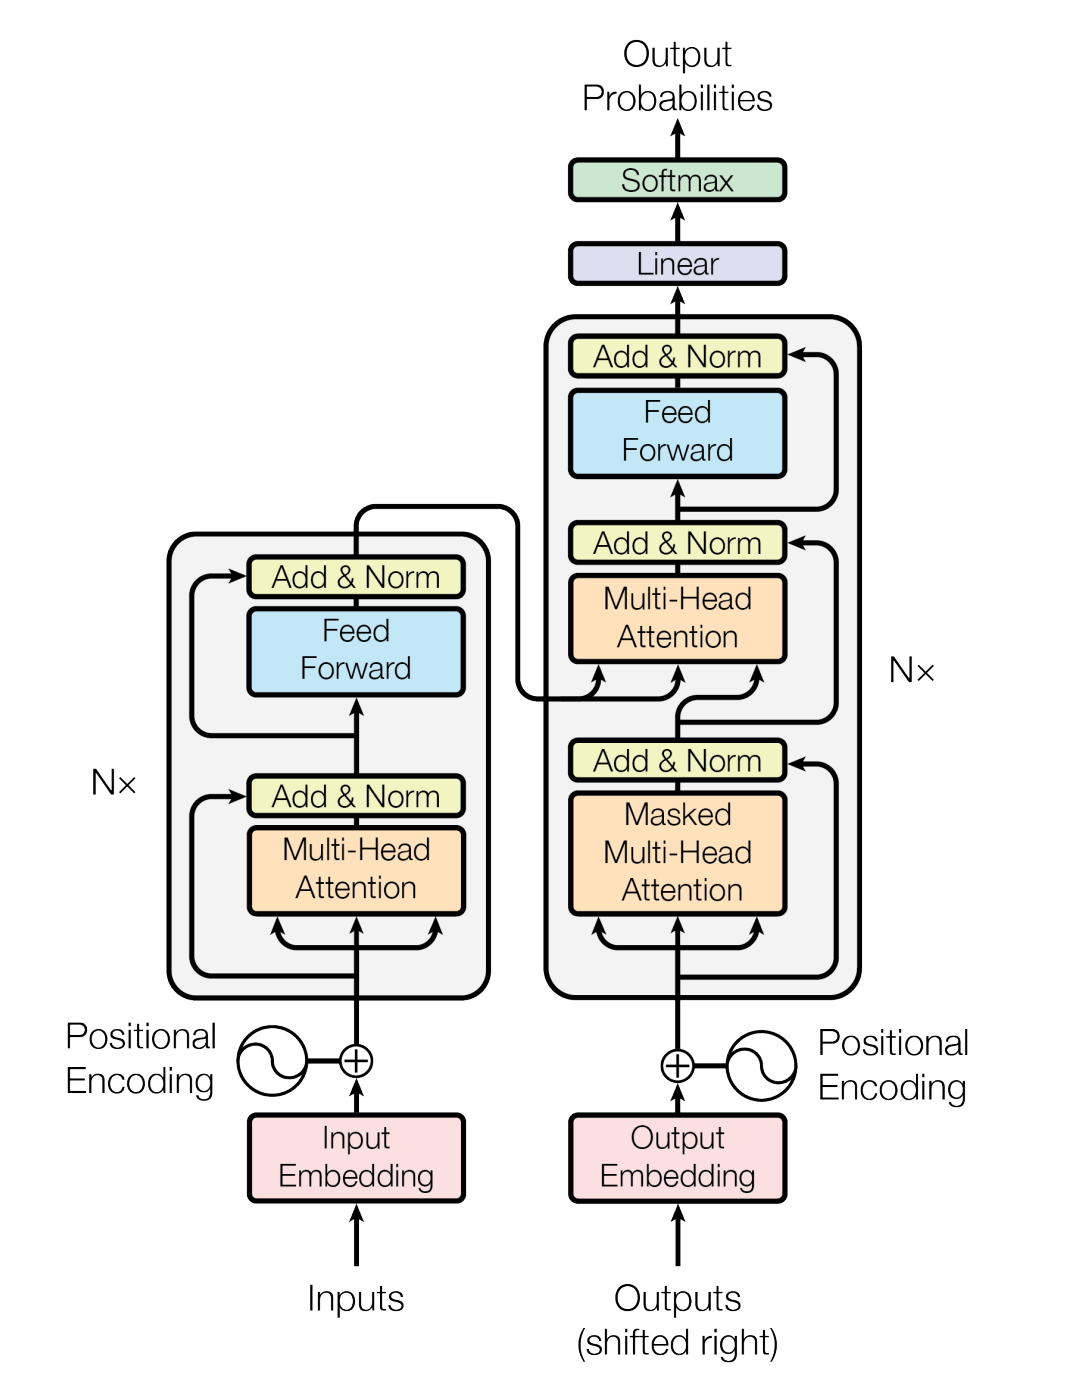
\includegraphics[width=16cm]{assets/Transformer.png}
    \caption[Transformerの概略図]{Transformerの概略図 (文献 \cite{Transformer} 図 1 参照)}
    \label{Transformer}
\end{figure}

\subsection{Bidirectional Encoder Representations from Transformers (BERT)}

Bidirectional Encoder Representations from Transformers (BERT) \cite{BERT} は, 2018 年に Google が発表した複数の双方向 Transformer に基づく汎用言語モデルである. BERT は, 入力された単語列全体と, 含まれる各単語に対応する分散表現を出力する. BERT は膨大なデータで教師なし学習をしたモデルである. これを各タスクに fine-tuning することでさまざまなタスクに柔軟に対応させることができる. \par
事前学習では, 膨大なデータを用いて Masked Language Modeling (MLM) と Next Sentence Prediction (NSP) の 2 つの教師なし学習が並行してなされる. 図 \ref{BERT_fine-tuning} に BERT の事前学習と転移学習の概略図を示す. \par
MLM は, 入力データの一部の単語を ``[MASK]" トークンに置き換えて BERT の入力として, 得られた各単語の分散表現から ``[MASK]" トークン部分の単語の元の単語を予測する学習方法である. ``[MASK]" がどの単語なのかを, 周辺の文脈から推定するタスクを解くことで, BERT は文脈を考慮した単語埋め込みを生成する能力を獲得する. しかし, ``[MASK]" というトークンは事前学習には登場するものの, fine-tuning の際にはタスクによっては登場せず, 事前学習と fine-tuning に乖離が生じてしまう. その問題を緩和するため, ``[MASK]" トークンに置き換えた単語に対して, 一定の確率で元の単語に戻し, また一定の確率でランダムな単語に置き換える. BERT が提案された論文においては, 全体の単語のうち 15\%を ``[MASK]" とし, 置き換えられた単語のうち 10\% を元の単語に戻し, 10\% をランダムな単語に置き換えている. \par
NSP は, 本来ならば文脈的に連続する 2 文の入力に対して, 一定の確率で不連続な 2 文に置き換えて, 得られた単語列全体の分散表現からその 2 文が連続しているかどうかを推定する学習方法である. 2 文の間の文脈を考慮してこのタスクを解くことで, BERT は, 文の交互関係が必要となるタスクを解く能力を獲得する. \par
これらの事前学習によって得られた BERT を fine-tuning することで, BERT は複数のタスクにおいて当時での最高峰精度を達成した. なお, BERT の登場以降, BERT はモデル構造に見合った性能を発揮できていないとして, BERT の訓練データを変え, 事前学習から NSP を除き, 動的マスキングをするなどの調整により, より良い精度を達成した RoBERTa \cite{RoBERT} や, BERT のモデルは肥大だとして, 推論能力をほとんど保持したままモデルサイズを大幅に減らした DistilBERT \cite{DistilBERT} といった, BERT に改良を加えたモデルが複数提案されている.\par

\begin{figure}[t]
    \centering
    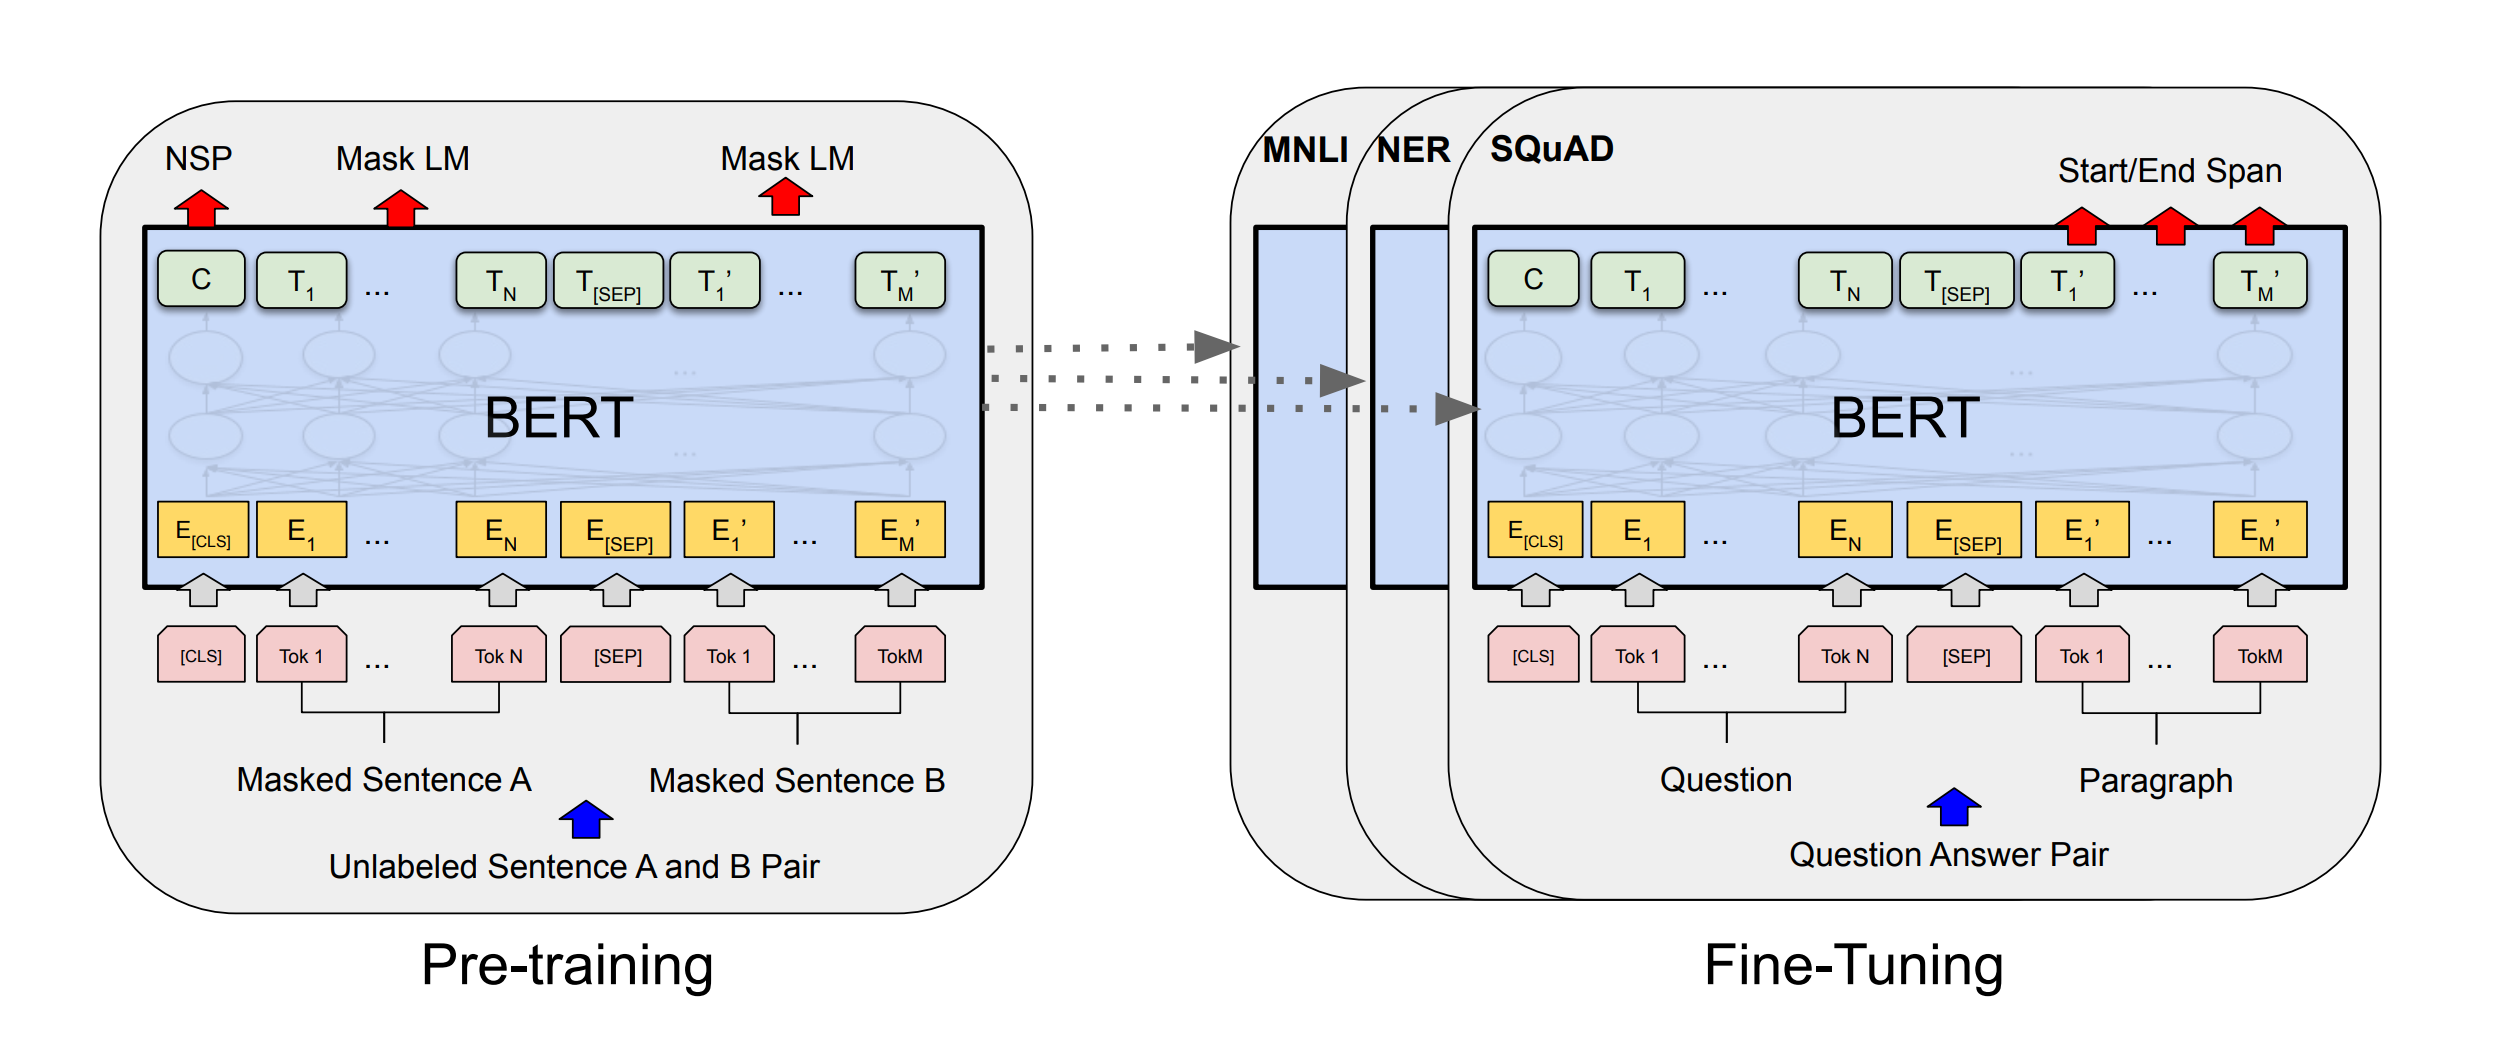
\includegraphics[width=16cm]{assets/BERT_fine-tuning.png}
    \caption[BERT の事前学習と転移学習の概略図]{BERT の事前学習と転移学習の概略図 (文献 \cite{BERT} 図 1 参照)}
    \label{BERT_fine-tuning}
\end{figure}

\subsection{Knowledge Graph BERT (KG-BERT)}

Knowledge Graph BERT (KG-BERT) \cite{KG-BERT} は, Yao らによって提案された BERT を fine-tuning することで Knowledge Graph を補完する手法である. 図 \ref{KG-BERT} に KG-BERT の概略図を示す. Entity と Relation はその名前や説明を単語のシーケンスとして表現し, それを入力文として BERT モデルを fine-tuning する. 文は実際の言語的な文ではなく, 任意の連続したテキストまたは単語のシーケンスである. Triple (Head, Relation, Tail) の文章を 1 つのシーケンスとしてまとめ, BERT への入力トークンシーケンスとして扱う. \par
図 \ref{KG-BERT} において, Tok はトークンを, $\bm{E}$, $\bm{T}$ は埋め込みベクトルとモデルの出力のベクトルをそれぞれ示す. $a, b, c$ は Head, Relation, Tail のトークン数を, h, r, t は Head, Relation, Tail をそれぞれ表す. 入力シーケンスの最初のトークンは常に特別なトークン ``[CLS]" である. Head Entity はトークン ${\rm Tok}_{1}^{\rm h}, …,{\rm Tok}_{a}^{\rm h}$ を含む文で表現され, Relation はトークン ${\rm Tok}_{1}^{\rm r}, …,{\rm Tok}_{b}^{\rm r}$ を含む文で表現され, Tail Entity はトークン ${\rm Tok}_{1}^{\rm t}, …,{\rm Tok}_{c}^{\rm t}$ を含む文で表現される. Entity と Relation の文は特別なトークン ``[SEP]" で区切られる. 同じ位置の異なるトークンは同じ位置埋め込みを共有し, ``[SEP]" で区切られた異なる要素は異なるセグメント埋め込みをもつ. 各入力トークンの入力表現は, 対応するトークン, セグメント, および位置埋め込みを合計して構築され, 異なる ``[SEP]" で区切られた要素は異なるセグメント埋め込みをもつ. 同じ位置 $i \in \{1, 2, 3, …, 512\}$ の異なるトークンは同じ位置埋め込みを共有する. 入力トークンの表現は, 元の BERT の実装に基づく多層双方向 Transformer エンコーダである BERT モデルアーキテクチャに供給される. 特別な ``[CLS]" トークンに対応する最終的な隠れベクトルと $i$ 番目の入力トークンの最終的な隠れベクトルは, それぞれ $\bm{C} \in \mathbb{R}^{H} $ および $\bm{T}_{i} \in \mathbb{R}^{H}$ で表される. ここで, $H$ は BERT における隠れベクトルのサイズである. ``[CLS]" に対応する最終的な隠れベクトル $C$ は, Triple スコアを計算するための集約シーケンス表現として使用される. Triple ${\rm \tau} = ({\rm h}, {\rm r}, {\rm t})$ のスコア関数は

\begin{equation}
\bm{s}_{\rm \tau} = f({\rm h}, {\rm r}, {\rm t}) = {\rm sigmoid}(CW^{\rm T})
\end{equation}

であり, $s_{\tau}$ は $s_{\tau0}, s_{\tau1} \in [0, 1]$ および $s_{\tau0} + s_{\tau1} = 1$ となる 2 次元の実ベクトルである. \par
正例の Triple セット $\mathbb{D}^{+}$ およびそれに応じて構築された負例の Triple セット $\mathbb{D}^{-}$ が与えられた場合, Triple のラベルに対するクロスエントロピー損失が計算される. 

\begin{equation}
    L = - \sum_{\tau \in \mathbb{D}^{+} \cup \mathbb{D}^{-}} (y_{\tau} \log{s_{\tau0}} + (1 - y_{\tau}) \log{s_{\tau1}})
\end{equation}

ラベル $y_{\tau} \in \{0, 1\}$ はその Triple のラベル (負または正) である. 負例の Triple セット $\mathbb{D}^{-}$ は, 正例の Triple (h, r, t) $\in \mathbb{D}^{+}$ の Head Entity h または Tail Entity t をランダムな Entity h' または t' で置き換えることで生成される. \par

\begin{equation}
    \begin{split} 
    \mathbb{D}^{-} = &\{ ({\rm h}', {\rm r}, {\rm t}) | {\rm h}' \in \mathbb{E} \land {\rm h}' \neq {\rm h} \land ({\rm h}', {\rm r}, {\rm t}) \notin \mathbb{D}^{+} \} \\ 
    &\cup \{ ({\rm h}, {\rm r}, {\rm t}') | {\rm t} \in \mathbb{E} \land {\rm t}' \neq {\rm t} \land ({\rm h}, {\rm r}, {\rm t}') \notin \mathbb{D}^{+} \}
    \end{split}
\end{equation}

ここで, E は Entity の集合である. 負例として扱うための条件は, その Triple が既に正例セット $\mathbb{D}^{+}$ に存在していない場合である. また, 事前に学習されたパラメータの重みと新しい重み $W \in \mathbb{R}^{2 \times H}$ は勾配降下法を使用して更新される. \par

\begin{figure}[h]
    \centering
    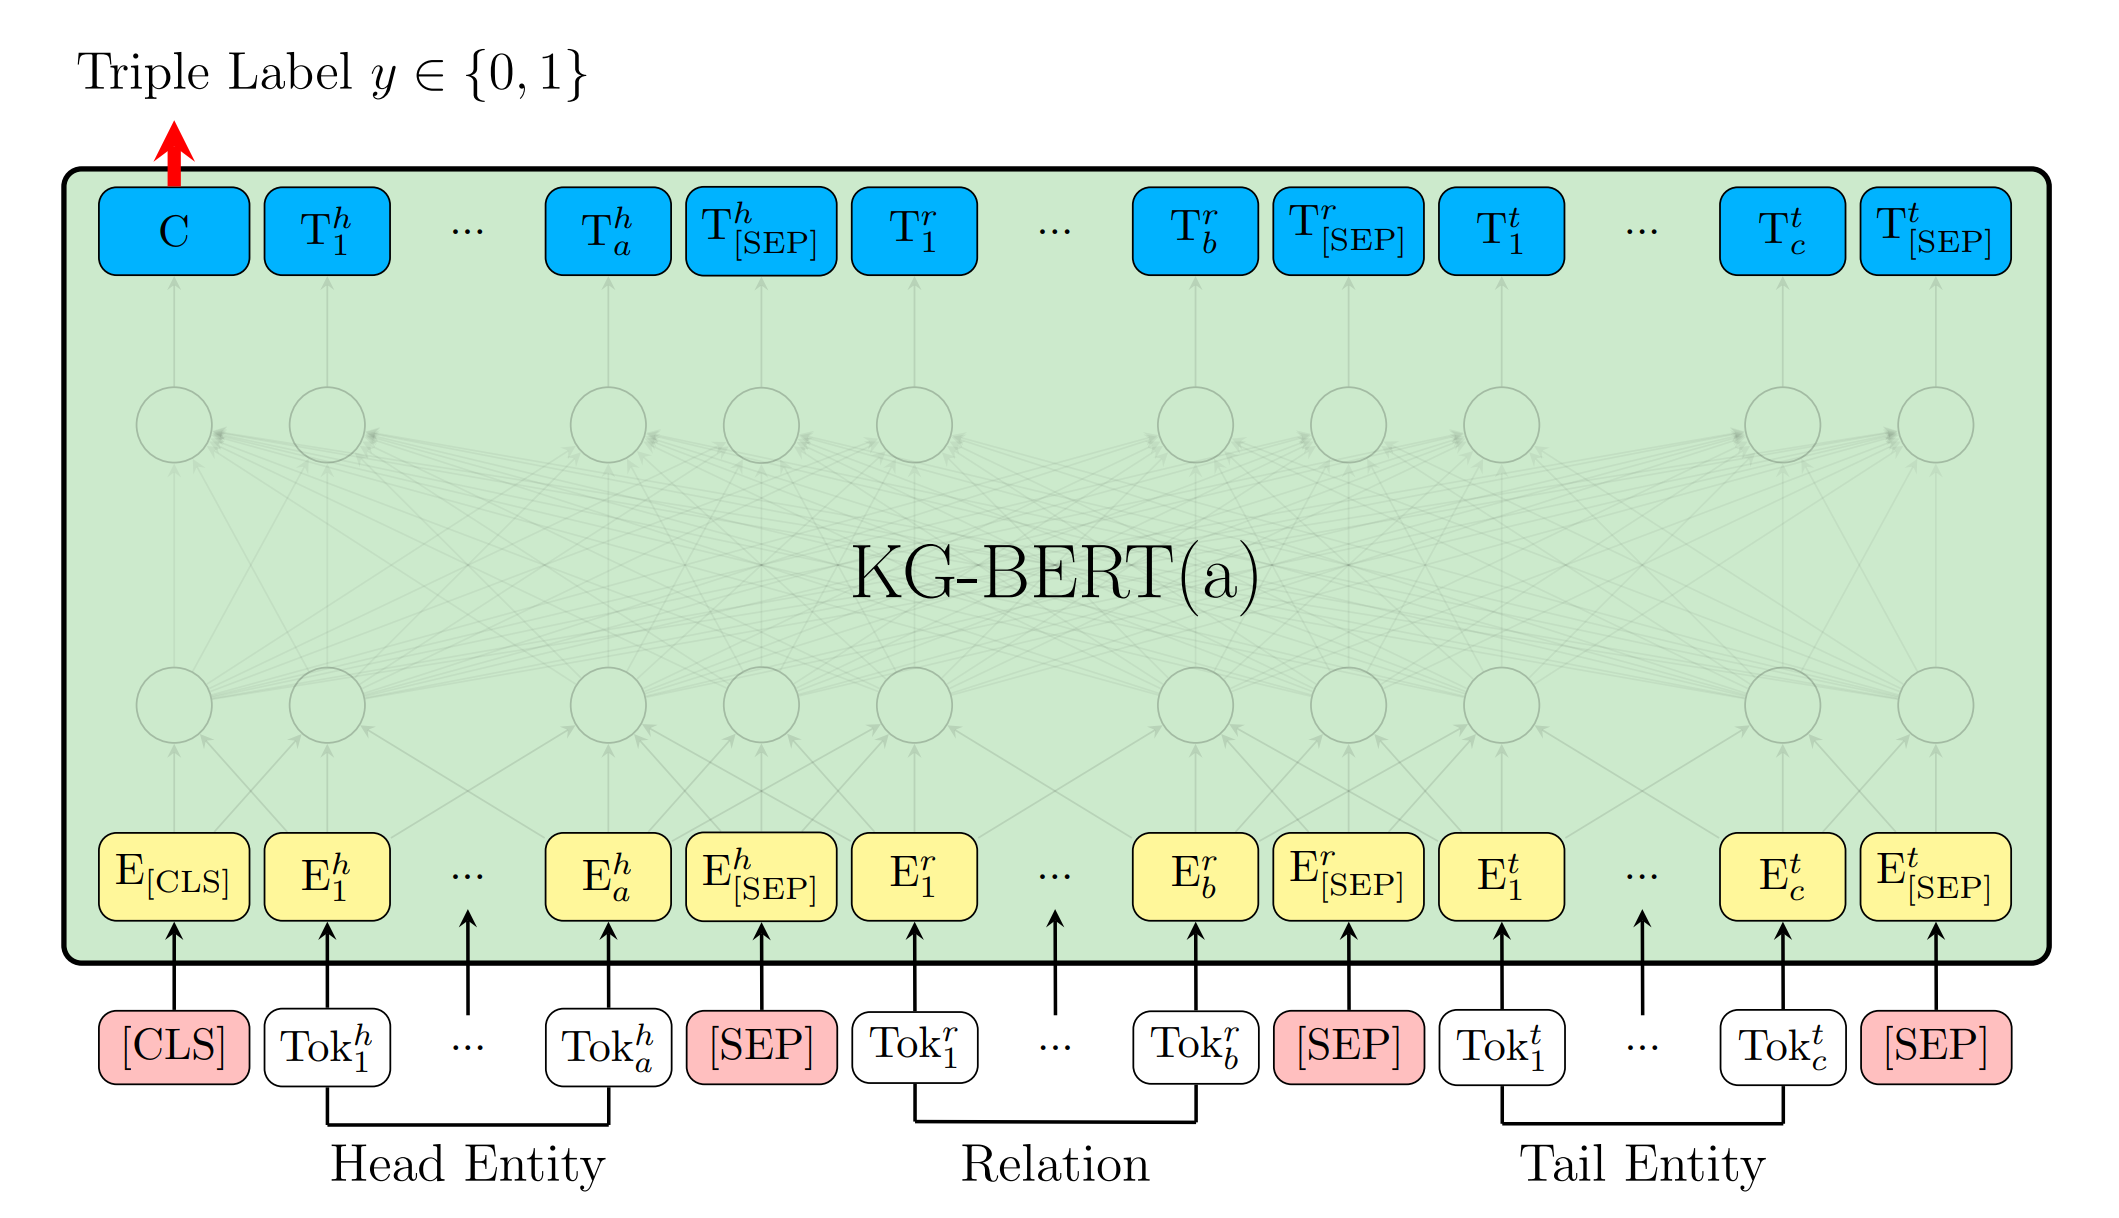
\includegraphics[width=16cm]{assets/KG-BERT.png}
    \caption[KG-BERT]{KG-BERT (文献 \cite{KG-BERT} 図 1 参照)}
    \label{KG-BERT}
\end{figure}

\subsection{WN18RR}

WN18RR \cite{WN18RR_ConvE} は, Dettmers らによって WordNet \cite{Wordnet} を基に作成された Triple のデータセットである. \par
WordNet は, 多言語で構成される大規模な語彙データベースであり, 単語同士の関係が品詞別に階層構造の形で格納されている.WordNet では Entity は単語の意味に対応し,Relation は Entity 間の語彙的な関係を表している.WordNet に含まれる関係の例として以下のものが挙げられる. \par

\begin{itemize}
      \item Synonymy (同義語)
      \item Hypernymy (上位語)
      \item Hyponymy (下位語)
      \item Holonymy (全体語)
      \item Meronymy (部分語)
\end{itemize}

WN18 \cite{TransE_WN18} は WordNet のサブセットであり, 18 種類の Relation と 40,943 種類の Entity で構成されている. WN18 には WordNet の Relation と Entity から作成された 151,442 個の Triple が存在し, その中に hyponym (下位語) の関係をもつ Triple と hypernym (上位語) の関係をもつ Triple が含まれている. このように, 階層構造となっている WN18 には逆関係の Triple が複数含まれている. そのため, WN18 では逆関係の Triple によるテスト漏洩の問題が生じる場合がある. 例えば, ある Relation r をもつ Triple (${\rm e}_{1}$, r, ${\rm e}_{2}$) とその逆関係の Triple (${\rm e}_{2}$, ${\rm r}'$, ${\rm e}_{1}$) が存在してそれぞれが訓練データ, テストデータに割り振られている場合, テストデータには訓練データに含まれる Triple と似ている Triple が存在することになる. \par
そこで, 逆関係のテスト漏洩がないデータセットとして WN18RR が作成された. WN18RR は WN18 から逆関係の Triple を除去して片方の Triple に統一したデータセットである. 表 \ref{example_wn18} に WN18 から逆関係の Triple を除去する例を示す. ある Relation r をもつ Triple (${\rm e}_{1}$, r, ${\rm e}_{2}$) とその逆関係の Triple (${\rm e}_{2}$, ${\rm r}'$, ${\rm e}_{1}$) の場合, Triple (${\rm e}_{1}$, r, ${\rm e}_{2}$) を残してその逆関係の Triple (${\rm e}_{2}$, ${\rm r}'$, ${\rm e}_{1}$) を除去する. これによって作成された WN18RR は 40,943 種類の Entity と 11 種類の Relation, 93,003 個の Triple をもつ. Entity はそれぞれ ``(見出し語), (説明文)" の形で表される. 表 \ref{example_Entity}, \ref{example_wn18rr} に WN18RR における Entity と Triple の例をそれぞれ示す. \par

\begin{table}[t]
    \centering
    \caption{WN18 から逆関係の Triple を除去する例}
    \label{example_wn18}
    \scalebox{1.0}{
    \begin{tabular}{|c||c|c|c|} \hline
      & Head & Relation & Tail \\ \hline \hline
      & poodle dog & hypernym & domestic dog \\ \hline
      除去& domestic dog & hyponym & poodle dog \\ \hline
      & telephone & hypernym & telecommunicate \\ \hline
      除去& telecommunicate & hyponym & telephone \\ \hline
      & home movie & hypernym & picture show \\ \hline
      除去& picture show & hyponym & home movie \\ \hline
      & \vdots & \vdots & \vdots \\ \hline
    \end{tabular}
    }
\end{table}

\begin{table}[t]
    \centering
    \caption{WN18RR における Entity の例}
    \label{example_Entity}
    \begin{tabular}{|cc|} \hline
      caption&description \\ \hline \hline
      poodle dog& an intelligent dog with a heavy curly solid-colored … \\ \hline
      domestic dog&a member of the genus Canis (probably descended … \\ \hline
      telephone&get or try to get into communication (with … \\ \hline
      wireless telephone&a telephone that communicates by radio waves … \\ \hline
      telephone set&electronic equipment that converts sound into … \\ \hline
      \multicolumn{2}{|c|}{\vdots} \\ \hline
    \end{tabular}
\end{table}

\begin{table}[t]
    \centering
    \caption{WN18RR における Triple の例}
    \label{example_wn18rr}
    \scalebox{1.0}{
    \begin{tabular}{|c|c|c|} \hline
      Head & Relation & Tail \\ \hline \hline
      telephone & hypernym & telecommunicate \\ \hline
      telephone system&has part&telephone set\\ \hline
      telephone system&has part&telephone exchange\\ \hline
      telephone system&hypernym&communication system \\ \hline
      telephone set&derivationally related form &telephone \\ \hline
      call&verb group&telephone \\ \hline
      cell phone&hypernym&telephone \\ \hline
      \vdots & \vdots & \vdots \\ \hline
    \end{tabular}
    }
\end{table}
